\chapter{Data Preparation and Model Training}
\label{chap:training}
The shape of the detector pulses is affected by many parameters, including particle energy, interaction position, charge cloud size, and so on. The relationship between the location of energy deposition and the resulting detector pulse is illustrated in Figure~\ref{fig:eng_dep_sim}. The left panel shows the interaction locations of particles within the detector for selected events. Event 3 and Event 4 are effectively single-sited, as the energy depositions occur very close to each other. In Event 1, the energy depositions result in two primary sites, giving rise to a two-sited pulse. Event 2 features a trace of energy deposition localized to three regions, classifying it as a three-sited event. 

\begin{figure}[htb!]
  %[trim={left bottom right top},clip]
    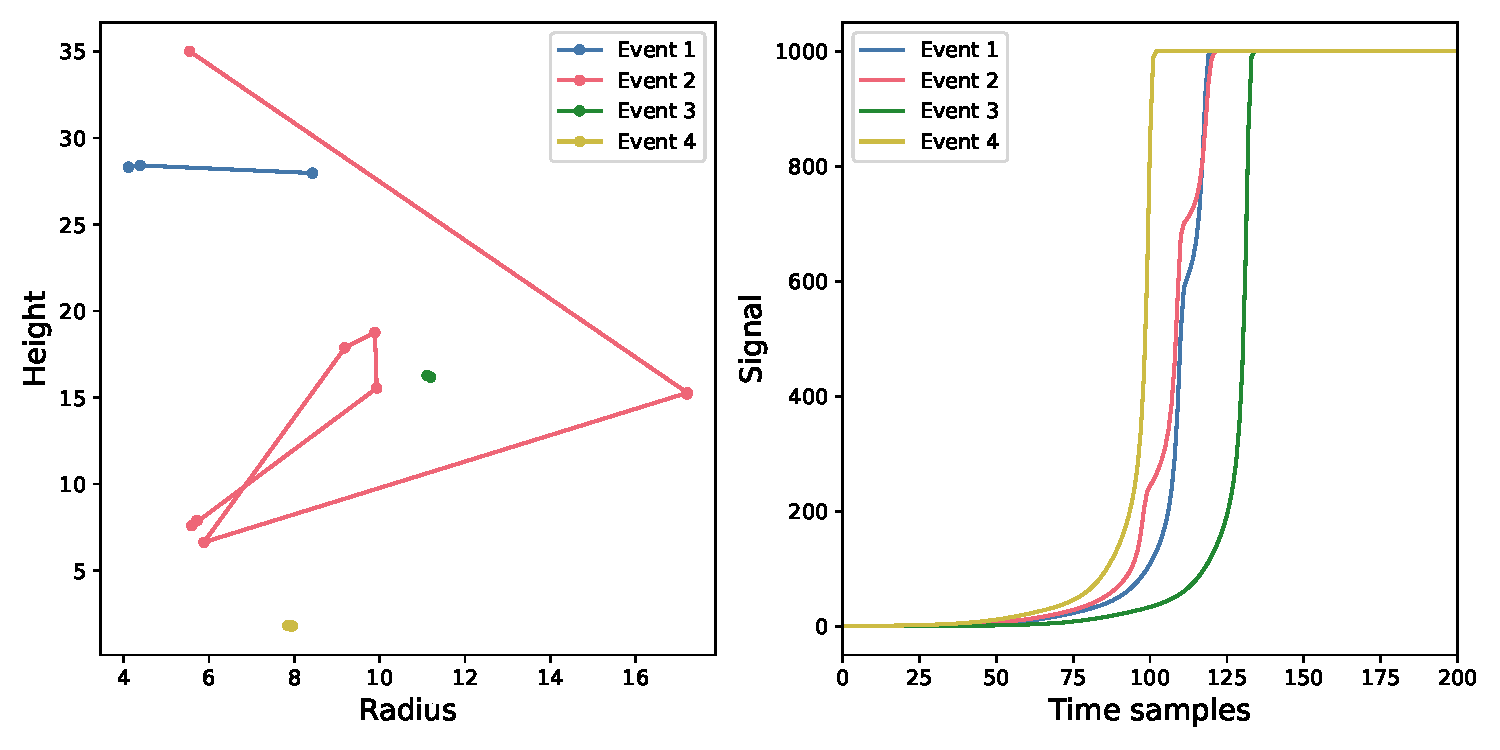
\includegraphics[width=0.99\linewidth,trim={1pc 0pc 1pc 0pc},clip]{ch6/figs/hits_and_pulses.pdf}
    \caption{(Left) Hit locations for each event. (Right) Energy-weighted pulses for the corresponding events. Hits produced using \texttt{Geant4} simulations and pulses generated using \texttt{siggen} software.}
   \label{fig:eng_dep_sim}
\end{figure}

\begin{figure}[htb!]
    % \hspace{0.05\linewidth}
    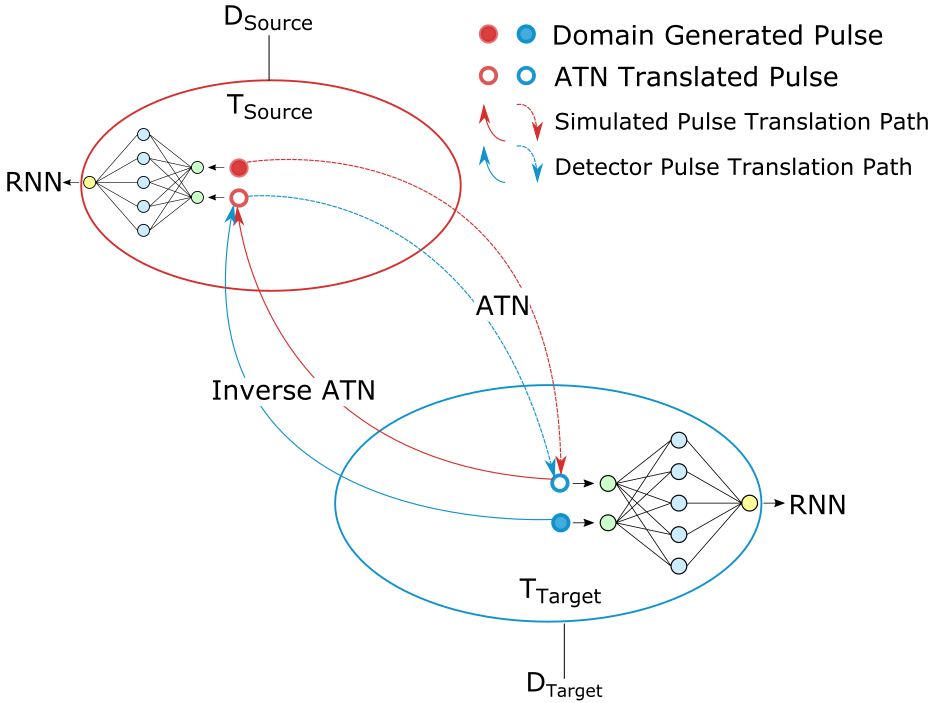
\includegraphics[width=0.99\linewidth]{ch6/figs/cycgan.png}
    \caption{Cycle-consistent adversarial training with PU-Net as the Ad-hoc Translation Network~(ATN) and Inverse Ad-hoc Translation Network~(IATN). The red oval region represents simulated pulses in $\mathcal{T}_{Source}$, and the blue oval region represents detector pulses in $\mathcal{T}_{Target}$.}
   \label{fig:network training}
\end{figure}